\documentclass[12pt]{article}
\usepackage{sbc-template}
\usepackage{graphicx}
\usepackage{amsmath}
\usepackage{subfigure}
\usepackage{times,amsmath,epsfig}
\usepackage{graphicx,url}
  \makeatletter
  \newif\if@restonecol
  \makeatother
  \let\algorithm\relax
  \let\endalgorithm\relax
\usepackage[lined,algonl,ruled]{algorithm2e}
\usepackage{multirow}
\usepackage[brazil]{babel}
\usepackage[utf8]{inputenc}
\usepackage[pdftex]{hyperref}

\sloppy

\title{Algoritmos e Estruturas de Dados 3 \\ Trabalho Prático 4 \\
\huge{CDFs! \\ Ordenação em memória externa}}
\date{November 22, 1963}


\author{André Taiar Marinho Oliveira}


\address{Departamento de Ciência da Computação -- Universidade Federal de Minas Gerais (UFMG)
\email{taiar@dcc.ufmg.br}
\\
\\ Novembro de 2010
}

\begin{document}

\maketitle

\begin{resumo}
Muitas aplicações em computação necessitam trabalhar com volumes de dados maiores do que
o que a memória principal (ou memória interna) das máquinas suporta. Tais aplicações precisam
fazer uso dos discos dos computadores que fornecem uma quantidade de espaço ordens de grandeza 
maior e suportam o volume de dados a ser computado, pagando para isso o preço da eficiência (dados 
em disco demoram ordens de grandeza de tempo a mais para serem acessados do que em memória interna).
Neste trabalho aplicaremos um método de ordenação em memória secundária para resolver o problema
das CDFs (\textit{Cumulative Distribution Function}) com um volume extenso de dados.
\end{resumo}

\section{Introdução}

A função de probabilidade acumulada (ou CDF) descreve completamente a
distribuição da probabilidade de uma variável aleatória de valor real $X$. 
Para cada número real $X$, a CDF é:

$F(x) = P(X =< x)$

Isso significa que, dado um número qualquer $X$ a CDF indica a probabilidade dos
outros valores $X$ serem menores ou iguais a $x$.

O algoritmo utilizado neste trabalho para calcular a CDF de um conjunto de
números em ponto flutuante é descrito no algoritmo \ref{alg:cdf}.

\begin{algorithm}[h!]
\label{alg:cdf}
\begin{footnotesize}
$D \longleftarrow $ conjunto muito grande de números (floats)\;
\tcp{Esta é a função mais importante deste trabalho.}
\textbf{ORDENA}$(D)$\; 
$count \longleftarrow$ 0\;
$current \longleftarrow$ $D[0]$\;
$len \longleftarrow$ TAMANHO$(D)$\;
\ForEach{$n \in D$}{
  \If{$n \neq current$}{
    $current \longleftarrow n$\;
    $prob \longleftarrow count/len$\;
    ESCREVE$(current, prob)$\;
  }
  $count \longleftarrow count + 1$\;
}
$n \longleftarrow D[len - 1]$\;
ESCREVE$(n, 1)$\;
\caption{Cálculo da CDF}
\end{footnotesize}
\end{algorithm}

O algoritmo de cálculo da CDF é bem simples, porém, como o volume de dados a ser
fornecido para ele é grande o suficiente para não caber na memória interna do
computador, isso faz com que o passo de ordenação dos dados se torne algo mais
complicado (necessita de ser ordenado na memória externa). Para cumprir essa parte
do trabalho, utilizaremos uma técnica chamada \textbf{Intercalação Balanceada de 
Vários Caminhos}.

\section{Solução Proposta}
\label{solucao_proposta}

O método de Intercalação Balanceada de Vários Caminhos, lê partes arbitrárias do 
aquivo de entrada a ser ordenado (partes essas que cabem em memória principal e 
podem ser manipuladas assim), as ordena e salva em arquivos temporários. Ao final 
do processo, quando todo o arquivo inicial está fragmentado em arquivos temporários
menores e ordenados, começa o processo de intercalação do algoritmo, onde os 
temporários são combinados na solução final obtendo-se o arquivo inicial ordenado.

Intercalar significa combinar dois ou mais blocos ordenados em um único bloco ordenado.
A intercalação, neste caso, é utilizada como uma operação auxiliar na ordenação. O 
processo completo utilizado para a ordenação neste trabalho é o visto no algoritmo 
\ref{alg:ord}.

\begin{algorithm}[h!]
\label{alg:ord}
\begin{footnotesize}

$file \longleftarrow$ aponta para o arquivo de entrada\;
$maxSize \longleftarrow$ máximo de valores a serem lidos\;
$v[maxSize] \longleftarrow$ vetor alocado com o tamanho de $maxSize$\;
$count \longleftarrow 0$\;
$tempId \longleftarrow 0$\;
\tcp{Gera temporários}
\While{houver dados em file}
{
	\While{$count < maxSize$}
	{
		$v[count] \longleftarrow$ READ$(file)$\;
		$count \longleftarrow count + 1$\;
	}
	ORDENA\_EM\_MEMORIA\_INTERNA($v$)\;
	ESCREVE\_TEMP($v, tempId$)\;
	$tempId \longleftarrow tempId + 1$\;
}
\tcp{Intercala}
$temps[tempId] \longleftarrow$ vetor alocado com o tamanho de $tempId$\;
\ForEach{arquivo temporário gerado $F_{i}$}
{
	$temps[i] \longleftarrow$ aponta para conteúdo do arquivo $F_{i}$\;
}
\While{houver dados em algum aquivo temporário $F_{i}$}
{
	$leitura \longleftarrow$ SELECIONA\_MENOR\_VALOR(temps);
	ESCREVE\_SAIDA($leitura$);
}

\caption{Intercalação Balanceada de Vários Caminhos}
\end{footnotesize}
\end{algorithm}

A quantidade máxima de valores a serem lidos a cada iteração na parte da geração
dos temporários foi limitada para efeitos de simulação em $1024 * 1024$ números.
Estes são salvos em um vetor e ordenados em memória interna utilizando o algoritmo
\textit{Quicksort}.

\section{Código}

\subsection{Módulos}
O programa foi separado em quatro módulos:
\begin{itemize}
\item \textbf{Entrada e Saída:} controla a leitura do arquivo de entrada
e a escrita do resultado no arquivo de saída. Também faz a validação dos 
argumentos de entrada pela linha de comando.
\item \textbf{Ordenação:} contém o método de ordenação em memória interna 
(\textit{Quicksort} recursivo).
\item \textbf{Externo:} contém o método de ordenação em memória externa. Utiliza
o módulo Ordenação para ordenar os arquivos parciais.
\item \textbf{Principal:} interagiu com todos os outros módulos retornando erro
quando alguma irregularidade era detectada, controla o fluxo de execução do
programa e mede o tempo de execução total do algoritmo.
\end{itemize}

\subsection{Entrada e saída}
\subsubsection{Linha de comando}
Para não haver problemas com a leitura da linha de comando, foi utilizado um utilitário do
sistema Linux chamado \textbf{getopt} que permite uma leitura mais robusta dos argumentos
passados ao programa. O comando para execução do programa definido para a linha de entrada 
foi:
\begin{verbatim}
#: ./tp4 -i <I> -o <O>
\end{verbatim}
Sendo: 
\begin{itemize}
  \item \textbf{I} - Arquivo de entrada;
  \item \textbf{O} - Arquivo de saída;
\end{itemize}

\subsubsection{Formato da entrada}
Para gerar o arquivo de entrada foi utilizado o script disponibilizado pelos monitores que 
gerava números em ponto flutuante com 15 casas de precisão. Os números devem ser positivos 
(pela própria especificação do problema). Não há restrição quanto à  precisão do número (o 
programa trata isso). Um exemplo de entrada válida seria:
\begin{verbatim}
180.00121515154
0.459887321
0.011115155511150
40.3333
40.3333
0.00001000
\end{verbatim}

\subsubsection{Formato da saída}
A saída do programa é retornada no arquivo de saída especificado pela linha de comando.
É formada por 2 colunas contendo na primeira os valores passados pela entrada, sem repetição
e ordenados e na segunda o valor da CDF calculada para o número da mesma linha na primeira 
coluna. O exemplo da saída gerada pela entrada descrita na sub-sessão anterior seria:
\begin{verbatim}
0.000010    0.00000
0.011115    0.00185
0.459887    0.07665
40.333300    6.72222
180.001215    1.00000
\end{verbatim}

Além disso o programa imprime na saída padrão quais foram os tempos de execução, usuário e sistema
gastos nessa execução:
\begin{verbatim}
tempo de execucao:  0.421001
tempo de usuario: 0.260000
tempo de sistema: 0.120000
\end{verbatim}

\subsubsection{Arquivos temporários e arquivo ordenado}
Para fazer a intercalação, vários arquivos temporários são gerados (dependendo do tamanho do arquivo
de entrada). Tais arquivos são nomeados com o prefixo \textit{"temp\_"} seguidos por um número inteiro
sequencial começando de $1$.

Além disso, ao intercalar os arquivos temporários é criado um arquivo de nome padrão (definido no código
do programa como "ordenado") com o conteúdo do arquivo de entrada ordenado com uma precisão de 5 casas decimais.

Todos os arquivos são gerados no diretório em que o executável se encontra.

\subsection{Compilação}
O compilador utilizado neste trabalho foi o GCC (adotado como padrão para a disciplina) e 
o comando para compilar o programa através do GCC é:
\begin{verbatim}
  #: gcc -o tp4 tp4.c io.c io.h externo.c externo.h ordena.c ordena.h
\end{verbatim}
caso estejam todos os arquivos dentro do mesmo diretório.

Como pedido na especificação, foi feito um arquivo Makefile com o qual é possível compilar
o programa com o comando: 
\begin{verbatim}
  #: make main
\end{verbatim}

E podemos compilar e executar o programa com o comando:
\begin{verbatim}
  #: make run
\end{verbatim}
que fará, além da compilação, com que o programa execute com uma entrada pequena.

\section{Avaliação Experimental}
\label{avaliacao_experimental}

Avaliamos experimentalmente os tempos de execução do programa variando o tamanho da entrada
de arquivos relativamente pequenos até valores que geralmente não cabem nas memórias internas 
dos computadores atuais. Todos os testes foram executados na máquina \textit{fourrier} na rede 
do DCC. Os resultados para os tempos de execução são mostrados na tabela \ref{tempossss} (tamanhos em megabytes 
e tempo em segundos):

\begin{table}[htb]
\centering
\caption{Tabela com os tempos de execução}
\label{tempossss}
\begin{tabular}{|c|c|c|c|}
\hline Tamanhos & Execução & Usuário & Sistema \\ 
\hline 10 & 4,26054320
 & 4,20000000
 & 0,05000000
 \\ 
\hline 50 & 20,93500840
 & 20,78199980
 & 0,14800000
 \\ 
\hline 100 & 41,11264280
 & 40,77800000
 & 0,28600000
 \\ 
\hline 500 & 205,77360860
 & 204,39200120
 & 1,17200000
 \\ 
\hline 1024 & 426,76674180
 & 423,85399780
 & 2,47200000
 \\ 
\hline 2048 & 876,34096680
 & 871,16400160
 & 4,60400000
 \\ 
\hline
\end{tabular} 
\end{table}

Os valores da tabela foram plotados na figura 1.

\begin{figure}[ht!]
\centering
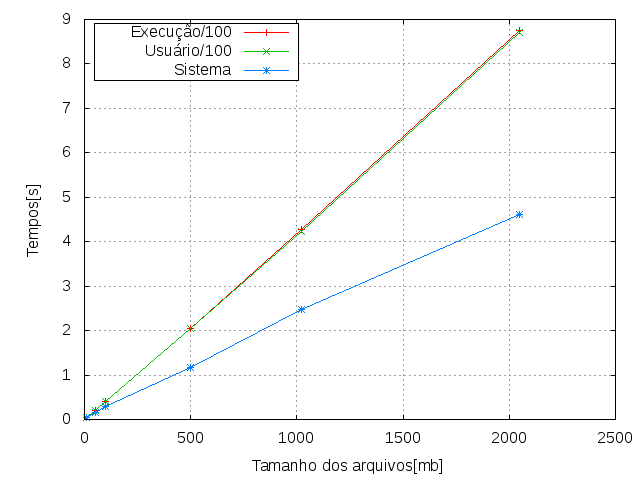
\includegraphics[width=3.5in,height=2.8in]{avali.png}
\label{img:resss}
\caption{Gráfico dos tempos de execução}
\end{figure}

\section{Conclusões}
\label{conclusao}



Algumas melhorias que poderiam ser consideradas neste trabalho são:
\begin{itemize}
\item Testar o passo de ordenação interna com outros algoritmos (Heapsort por exemplo - por
ser mais estável que o Quicksort);
\item Analisar o comportamento do programa para diferentes tamanhos de memória (variar o 
número de itens a serem lidos e ordenados em memória inteira);
\item A utilização de paralelismo de dados ou de tarefas poderia ser muito interessante na resolução desse problema uma vez que um grande se encontra no passo da ordenação interna.
\end{itemize}

\end{document}
